\documentclass{book}
\usepackage[shortlabels]{enumitem}
\usepackage{amsmath}
\usepackage{amssymb}
\usepackage{marvosym}
\let\marvosymLightning\Lightning

\usepackage{pgfplots}
\usepgfplotslibrary{fillbetween}

\newcommand{\mathcolorbox}[2]{\colorbox{#1}{$\displaystyle #2$}}

\newtheorem{definition}{Definition}

\begin{document}

\chapter{Funktionsuntersuchung}

\section{Grundtypen von Funktionen}

\begin{enumerate}[a)]

\item Potenzfunktionen

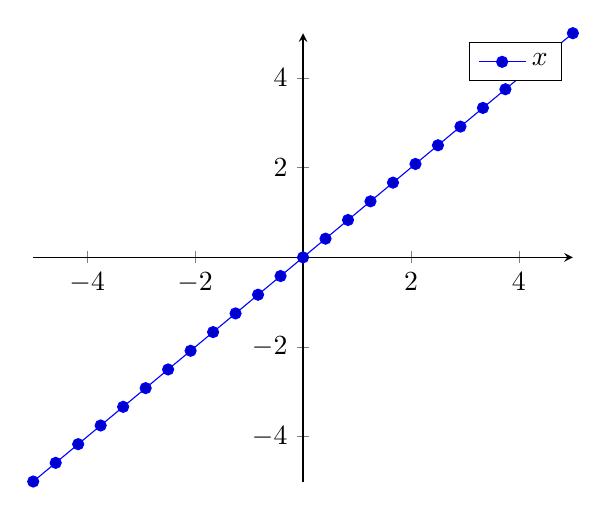
\begin{tikzpicture}
\begin{axis}[axis lines = middle]
\addplot{x};
\addlegendentry{\( x\)}
\end{axis}
\end{tikzpicture}

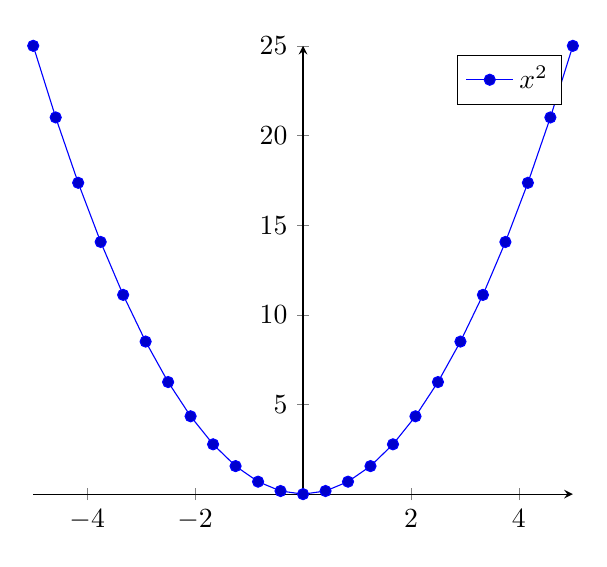
\begin{tikzpicture}
\begin{axis}[axis lines = middle]
\addplot{x^2};
\addlegendentry{\( x^2\)}
\end{axis}
\end{tikzpicture}

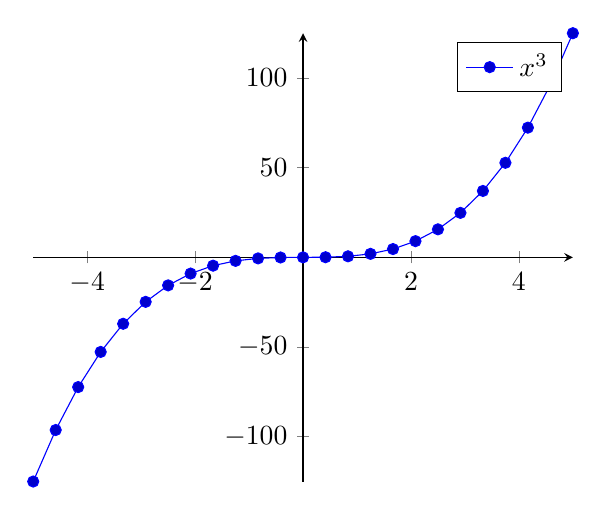
\begin{tikzpicture}
\begin{axis}[axis lines = middle]
\addplot{x^3};
\addlegendentry{\( x^3\)}
\end{axis}
\end{tikzpicture}

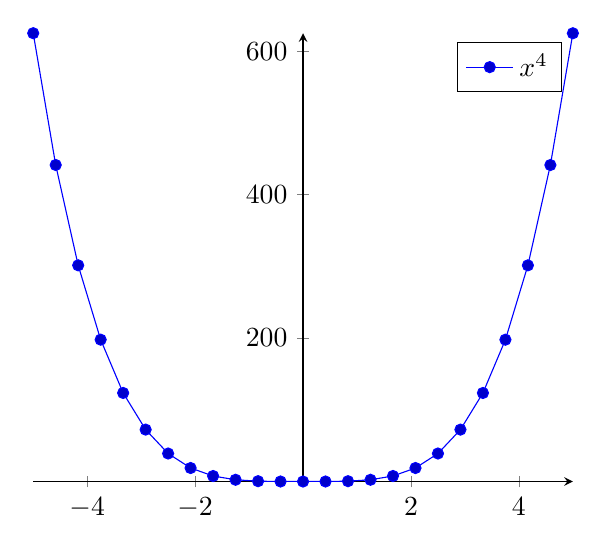
\begin{tikzpicture}
\begin{axis}[axis lines = middle]
\addplot{x^4};
\addlegendentry{\( x^4\)}
\end{axis}
\end{tikzpicture}

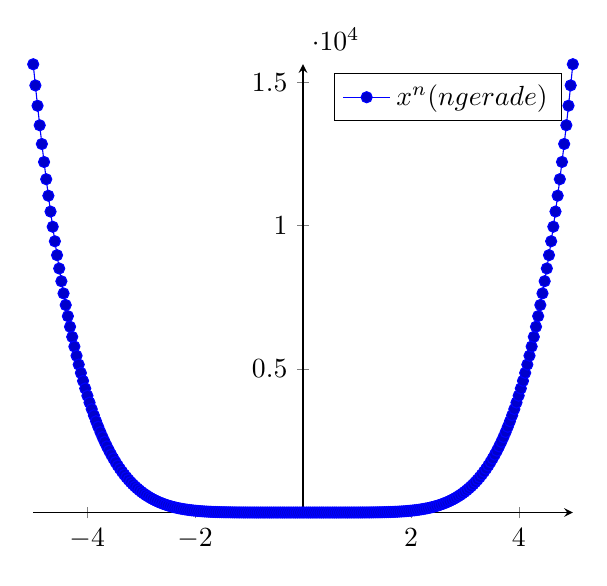
\begin{tikzpicture}
\begin{axis}[axis lines = middle, samples=250]
\addplot{x^6};
\addlegendentry{\( x^n (n gerade)\)}
\end{axis}
\end{tikzpicture}

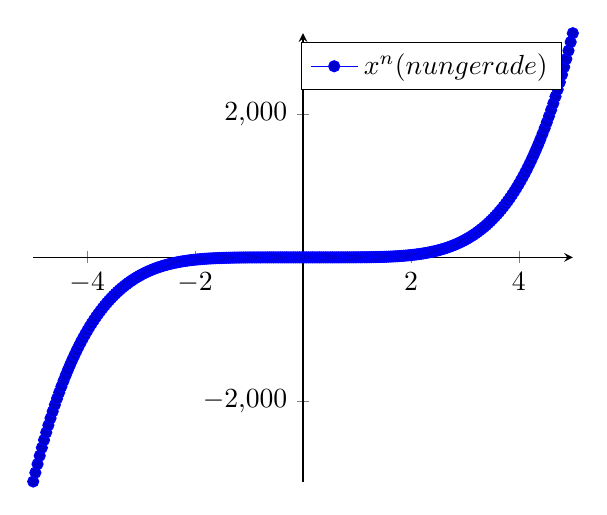
\begin{tikzpicture}
\begin{axis}[axis lines = middle, samples=250]
\addplot{x^5};
\addlegendentry{\( x^n (n ungerade)\)}
\end{axis}
\end{tikzpicture}

\item Würzelfunktionen

\begin{tikzpicture}
\begin{axis}[axis lines = middle]
\addplot{sqrt(x)};
\addlegendentry{\( \sqrt x\)}
\end{axis}
\end{tikzpicture}

\item Exponential Funktionen

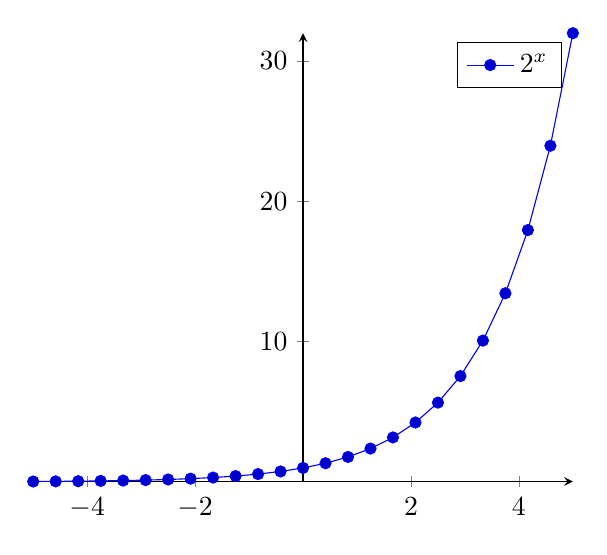
\begin{tikzpicture}
\begin{axis}[axis lines = middle]
\addplot{2^x};
\addlegendentry{\( 2^x \)}
\end{axis}
\end{tikzpicture}

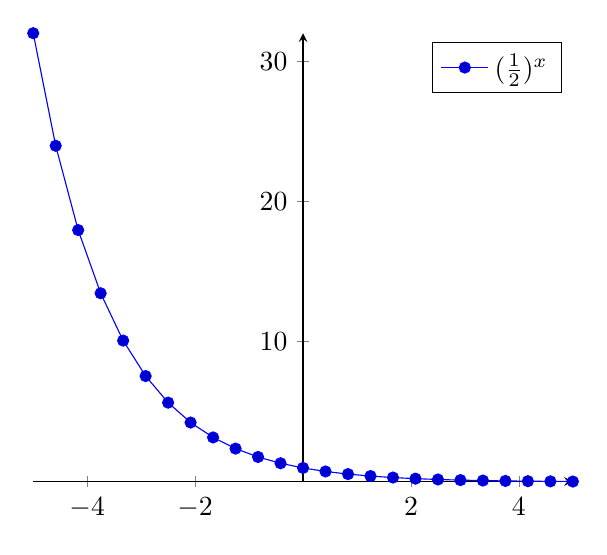
\begin{tikzpicture}
\begin{axis}[axis lines = middle]
\addplot{(1/2)^x};
\addlegendentry{\( (\frac 12)^x \)}
\end{axis}
\end{tikzpicture}


\item Gebrodenrationale Funktionen

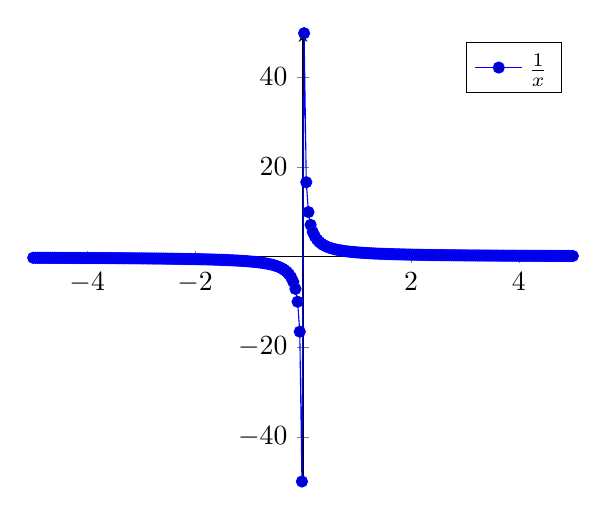
\begin{tikzpicture}
\begin{axis}[axis lines = middle, samples = 250] %, title=$f(x) = \frac {1}{x}$
\addplot{1/x};
\addlegendentry{\( \frac 1 x\)}
\end{axis}
\end{tikzpicture}

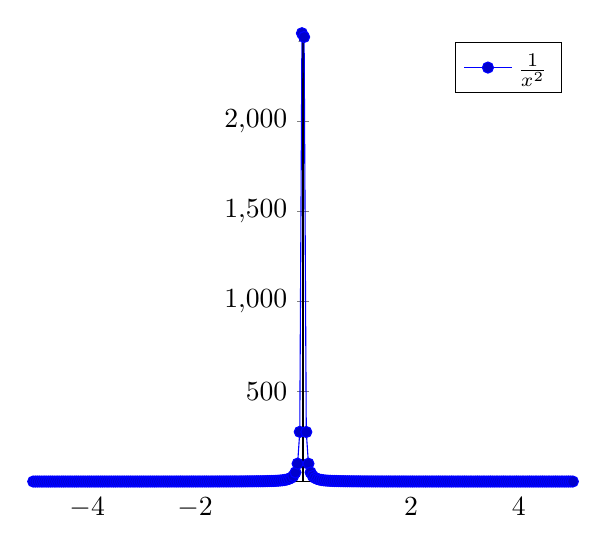
\begin{tikzpicture}
\begin{axis}[axis lines = middle, samples = 250] % , title=$g(x) = \frac 1{x^2}$
\addplot{1/(x^2)};
\addlegendentry{\( \frac 1 {x^2} \)}
\end{axis}
\end{tikzpicture}

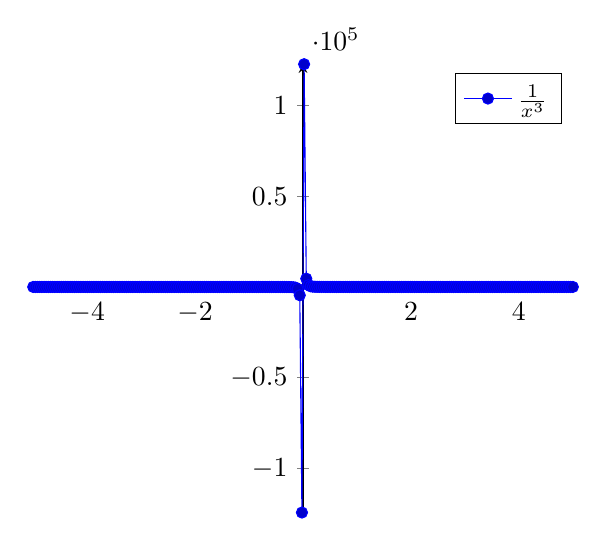
\begin{tikzpicture}
\begin{axis}[axis lines = middle, samples = 250]
\addplot{1/(x^3)};
\addlegendentry{\( \frac 1{x^3}\)}
\end{axis}
\end{tikzpicture}

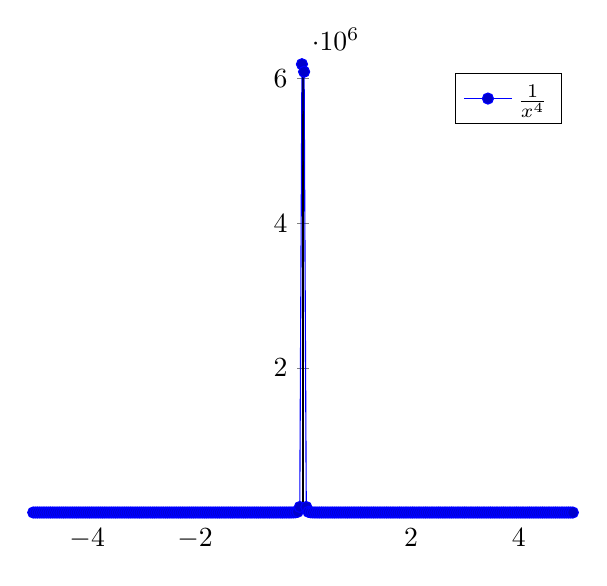
\begin{tikzpicture}
\begin{axis}[axis lines = middle, samples = 250]
\addplot{1/(x^4)};
\addlegendentry{\(\frac1{x^4}\)}
\end{axis}
\end{tikzpicture}

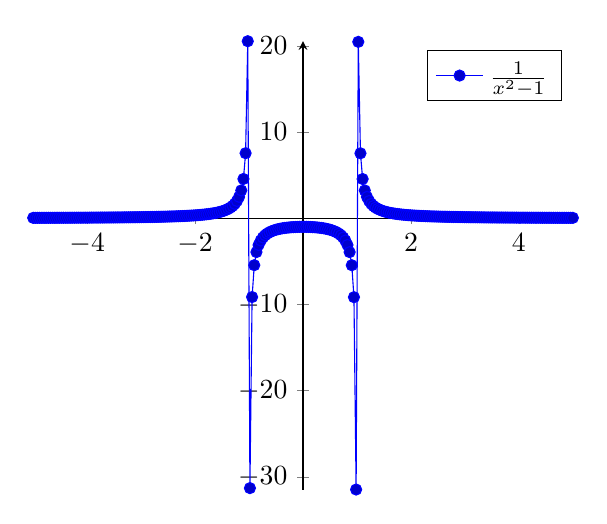
\begin{tikzpicture}
\begin{axis}[axis lines = middle, samples = 250]
\addplot{1/(x^2-1)};
\addlegendentry{\(\frac1{x^2-1}\)}
\end{axis}
\end{tikzpicture}

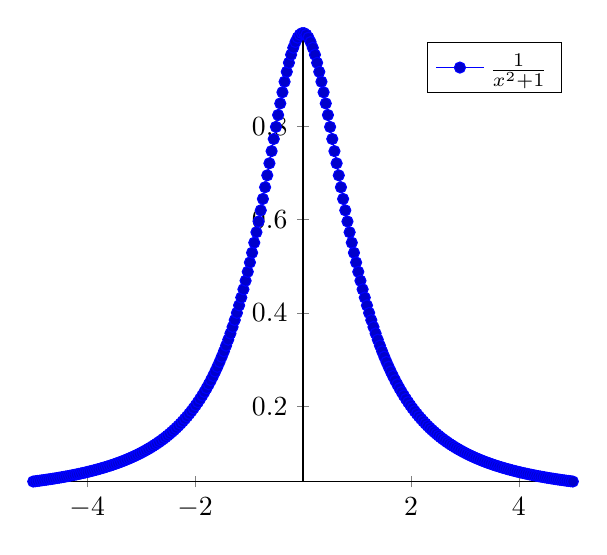
\begin{tikzpicture}
\begin{axis}[axis lines = middle, samples = 250] % , title=$f(x) = $
\addplot{1/(x^2+1)};
\addlegendentry{\(\frac 1{x^2+1}\)}
\end{axis}
\end{tikzpicture}


\item Trigonometrische Funktionen

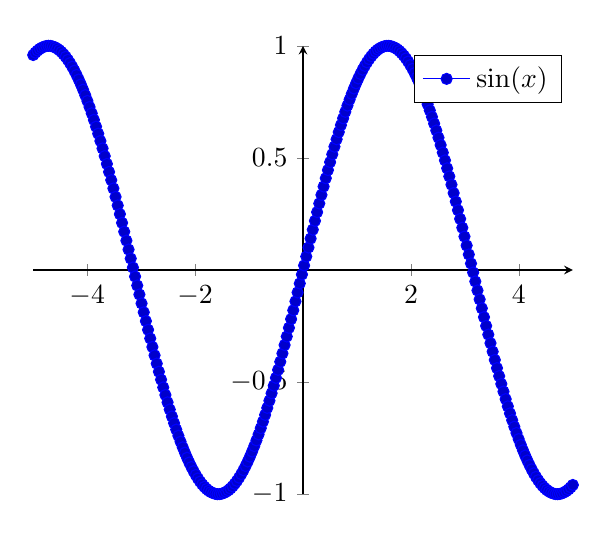
\begin{tikzpicture}
\begin{axis}[axis lines = middle, samples=250] % , title=$f(x) = $
\addplot{sin(deg(x))};\
\addlegendentry{$\sin(x)$}
\end{axis}
\end{tikzpicture}

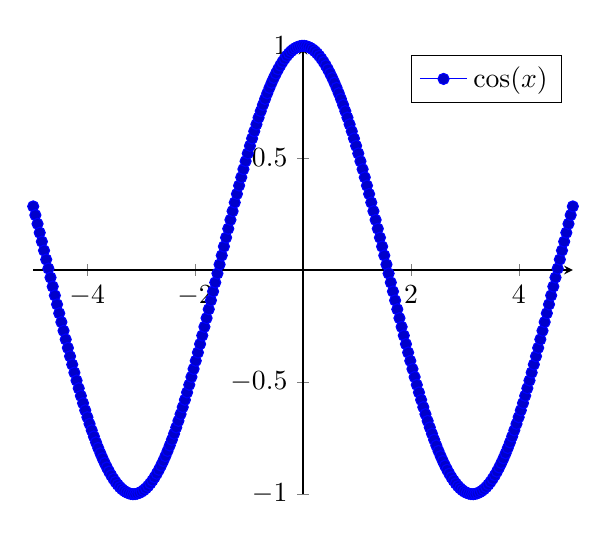
\begin{tikzpicture}
\begin{axis}[axis lines = middle, samples=250] % , title=$f(x) = \cos(x)$
\addplot{cos(deg(x))};
\addlegendentry{\(\cos(x)\)}
\end{axis}
\end{tikzpicture}

\item Betragsfunktionen

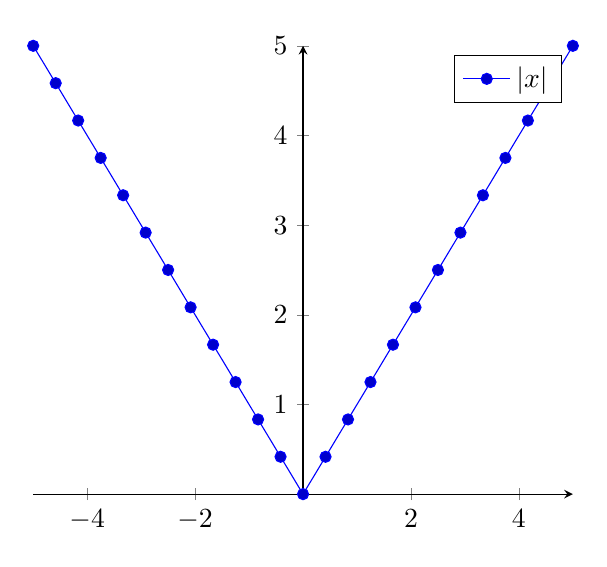
\begin{tikzpicture}
\begin{axis}[axis lines = middle] % , title=$f(x) = \cos(x)$
\addplot{abs(x)};
\addlegendentry{\(|x|\)}
\end{axis}
\end{tikzpicture}

\item Logarithmusfunktionen zur Basis e

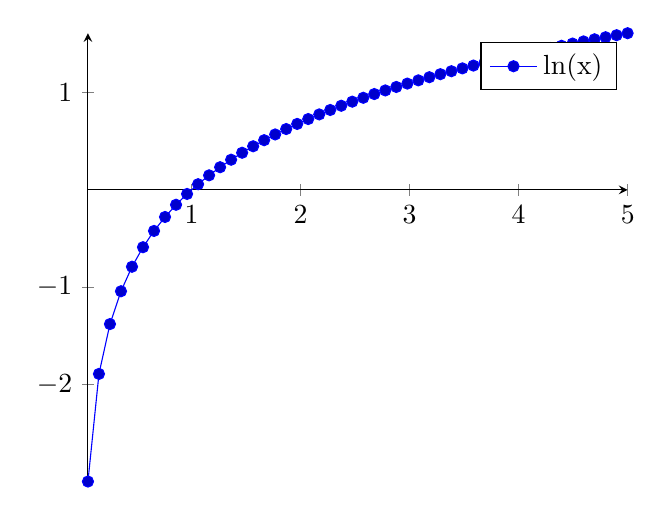
\begin{tikzpicture}
\begin{axis}[axis lines = middle, samples = 100]
\addplot{ln(x)};
\addlegendentry{ln(x)}
\end{axis}
\end{tikzpicture}

\end{enumerate}

\section{Operationen an Funktionen}

\[g(x) = a \cdot f(b\cdot x-c) + d, \; a, b, c, d \in \mathbb{R} ; \; a\not = 0\]

\subsection{Streckung}
\begin{itemize}[-]
\item y-Richtung mit dem Faktor a: $f(x) = a \cdot g(x)$
\item x-Richtung mit dem Faktor b: $f(x) = g(b\cdot x)$

\end{itemize}
\subsection{Verschiebung}

\begin{itemize}[-]
\item y-Richtung mit dem Faktor d: $f(x) = g(x) + d $

\item x-Richtung mit dem Faktor c: $f(x) = g(x+c) $
\end{itemize}

\subsection{Spiegeln}

\begin{itemize}[-]
\item y-Achse $f(x) = g(-x)$
\item x-Achse $f(x) = -g(x)$
\item Ursprung $f(x) = -g(-x)$
\end{itemize}

\section {Abbildung von Funktionen}

\[f(x) = \frac a {b(x-c)^2} +d\]
\begin{itemize}[-]
\item a y Streckung
\item b x Streckung
\item c x Verschiebung
\item d y Verschiebung
\end{itemize}


\end{document}
